\documentclass{beamer}
\setbeamercovered{transparent}
\usepackage{epstopdf}
\usepackage{listings}
\usepackage{lipsum}
\usepackage{subfig}
\usepackage{algorithm}
\usepackage{algorithmicx}
\usepackage{cite}
\usepackage{lipsum}
\usepackage{amssymb}
\usepackage{color}
\usepackage{IEEEtrantools}
\usepackage{booktabs}
\usepackage{texpower}
\usepackage{amsmath}
\usepackage{caption}
\usepackage{multirow}
\usepackage{graphicx}
\newtheorem{Key points}{Key points}
\newtheorem{Summary}{Summary}
\usepackage{dblfloatfix}
%\usepackage{adjustbox}
%\usepackage{animate}
%\usepackage{movie15}
%\usepackage{subfig}
%\newtheorem{Definition}{Definition}
%\usepackage[font={small}]{caption}
\usepackage{beamerthemeshadow}
\newcommand\Fontvi{\fontsize{5}{6.2}\selectfont}
\newcommand\Fontvia{\fontsize{6}{7.2}\selectfont}
\newcommand\Fontviaa{\fontsize{8}{7.2}\selectfont}
\usepackage{listings}
\lstset{language=C++,
                keywordstyle=\color{blue},
                stringstyle=\color{red},
                commentstyle=\color{green},
                morecomment=[l][\color{magenta}]{\#},
                numbers=left,
                escapeinside=||
}

%\captionsetup{font=scriptsize,labelfont=scriptsize}
 \usetheme{Antibes}%PaloAlto
\begin{document}
\title[Lecture 4]{Data Structures and Object Oriented Programming using C++} 
\author[]{Ahsan Ijaz}
\date{}
 \frame{\titlepage}
% \AtBeginSection[]
% {
% \begin{frame}<beamer>{Table of Contents}
% \tableofcontents[currentsection,currentsubsection, 
%     hideothersubsections, 
%     sectionstyle=show/shaded,
% ]
% \end{frame}
% }
\section{Review of Last Lecture}
\frame{\frametitle{Topics Covered}
  \begin{itemize}
  \item<1-> Classes
  \item<2-> Objects
  \item<3-> Data Hiding
  \item<4-> Constructors
  \item<5-> Destructors
  \item<6-> Namespaces
  \end{itemize}
}

\section{Quiz\#1 Hall of Fame}
\frame{\frametitle{Hall of Fame}
\begin{itemize}
\item {\color{blue}Uzair Arshad}
\item {\color{blue}Afeef Ahmed}
\item {\color{blue}Ayesha Sarwar}
\item {\color{blue}Bashir-ud-Din}
\item {\color{blue}Hassan Hashmi}
\item {\color{blue}Zohaib Shabir}
\item {\color{red}Shahzaib}
\item {\color{red}Waleed Ahmed}
\end{itemize}
}
\frame{\frametitle{Sample Quiz 1}
  \begin{figure}
    \centering
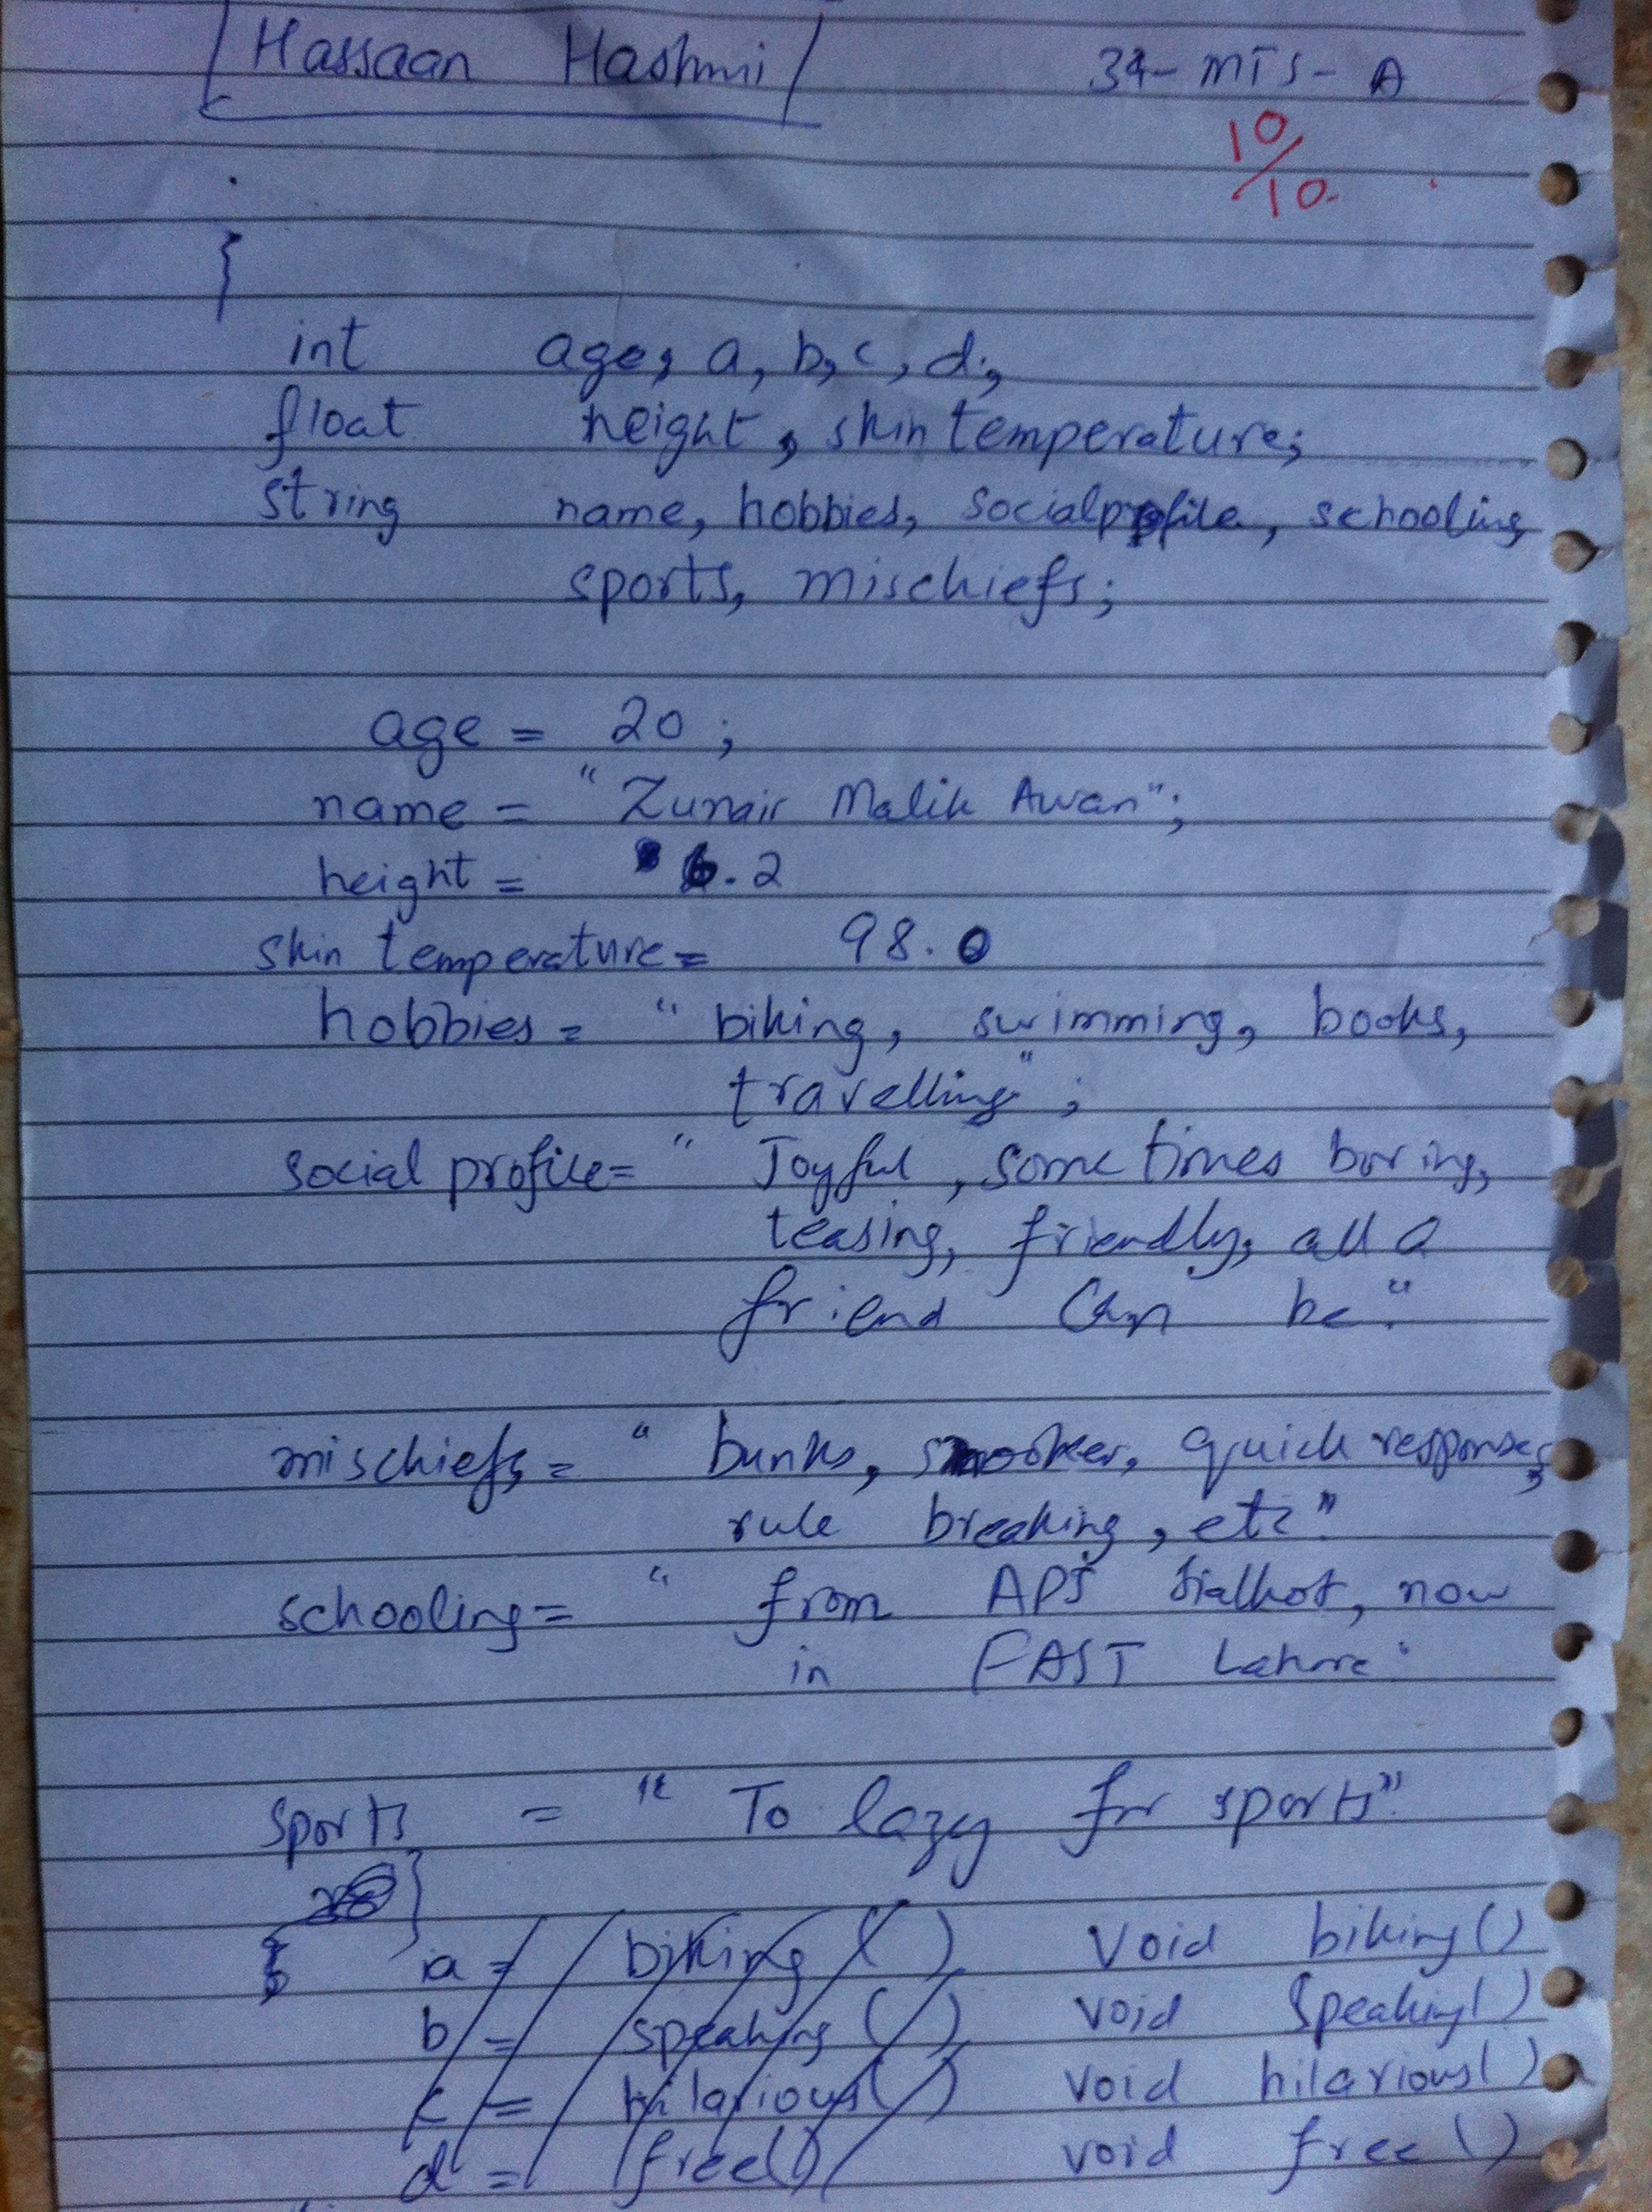
\includegraphics[width=0.4\columnwidth]{hashmi}    
\caption{Hassan Hashmi}
  \end{figure}

}
\frame{\frametitle{Sample Quiz 2}
  \begin{figure}
    \centering
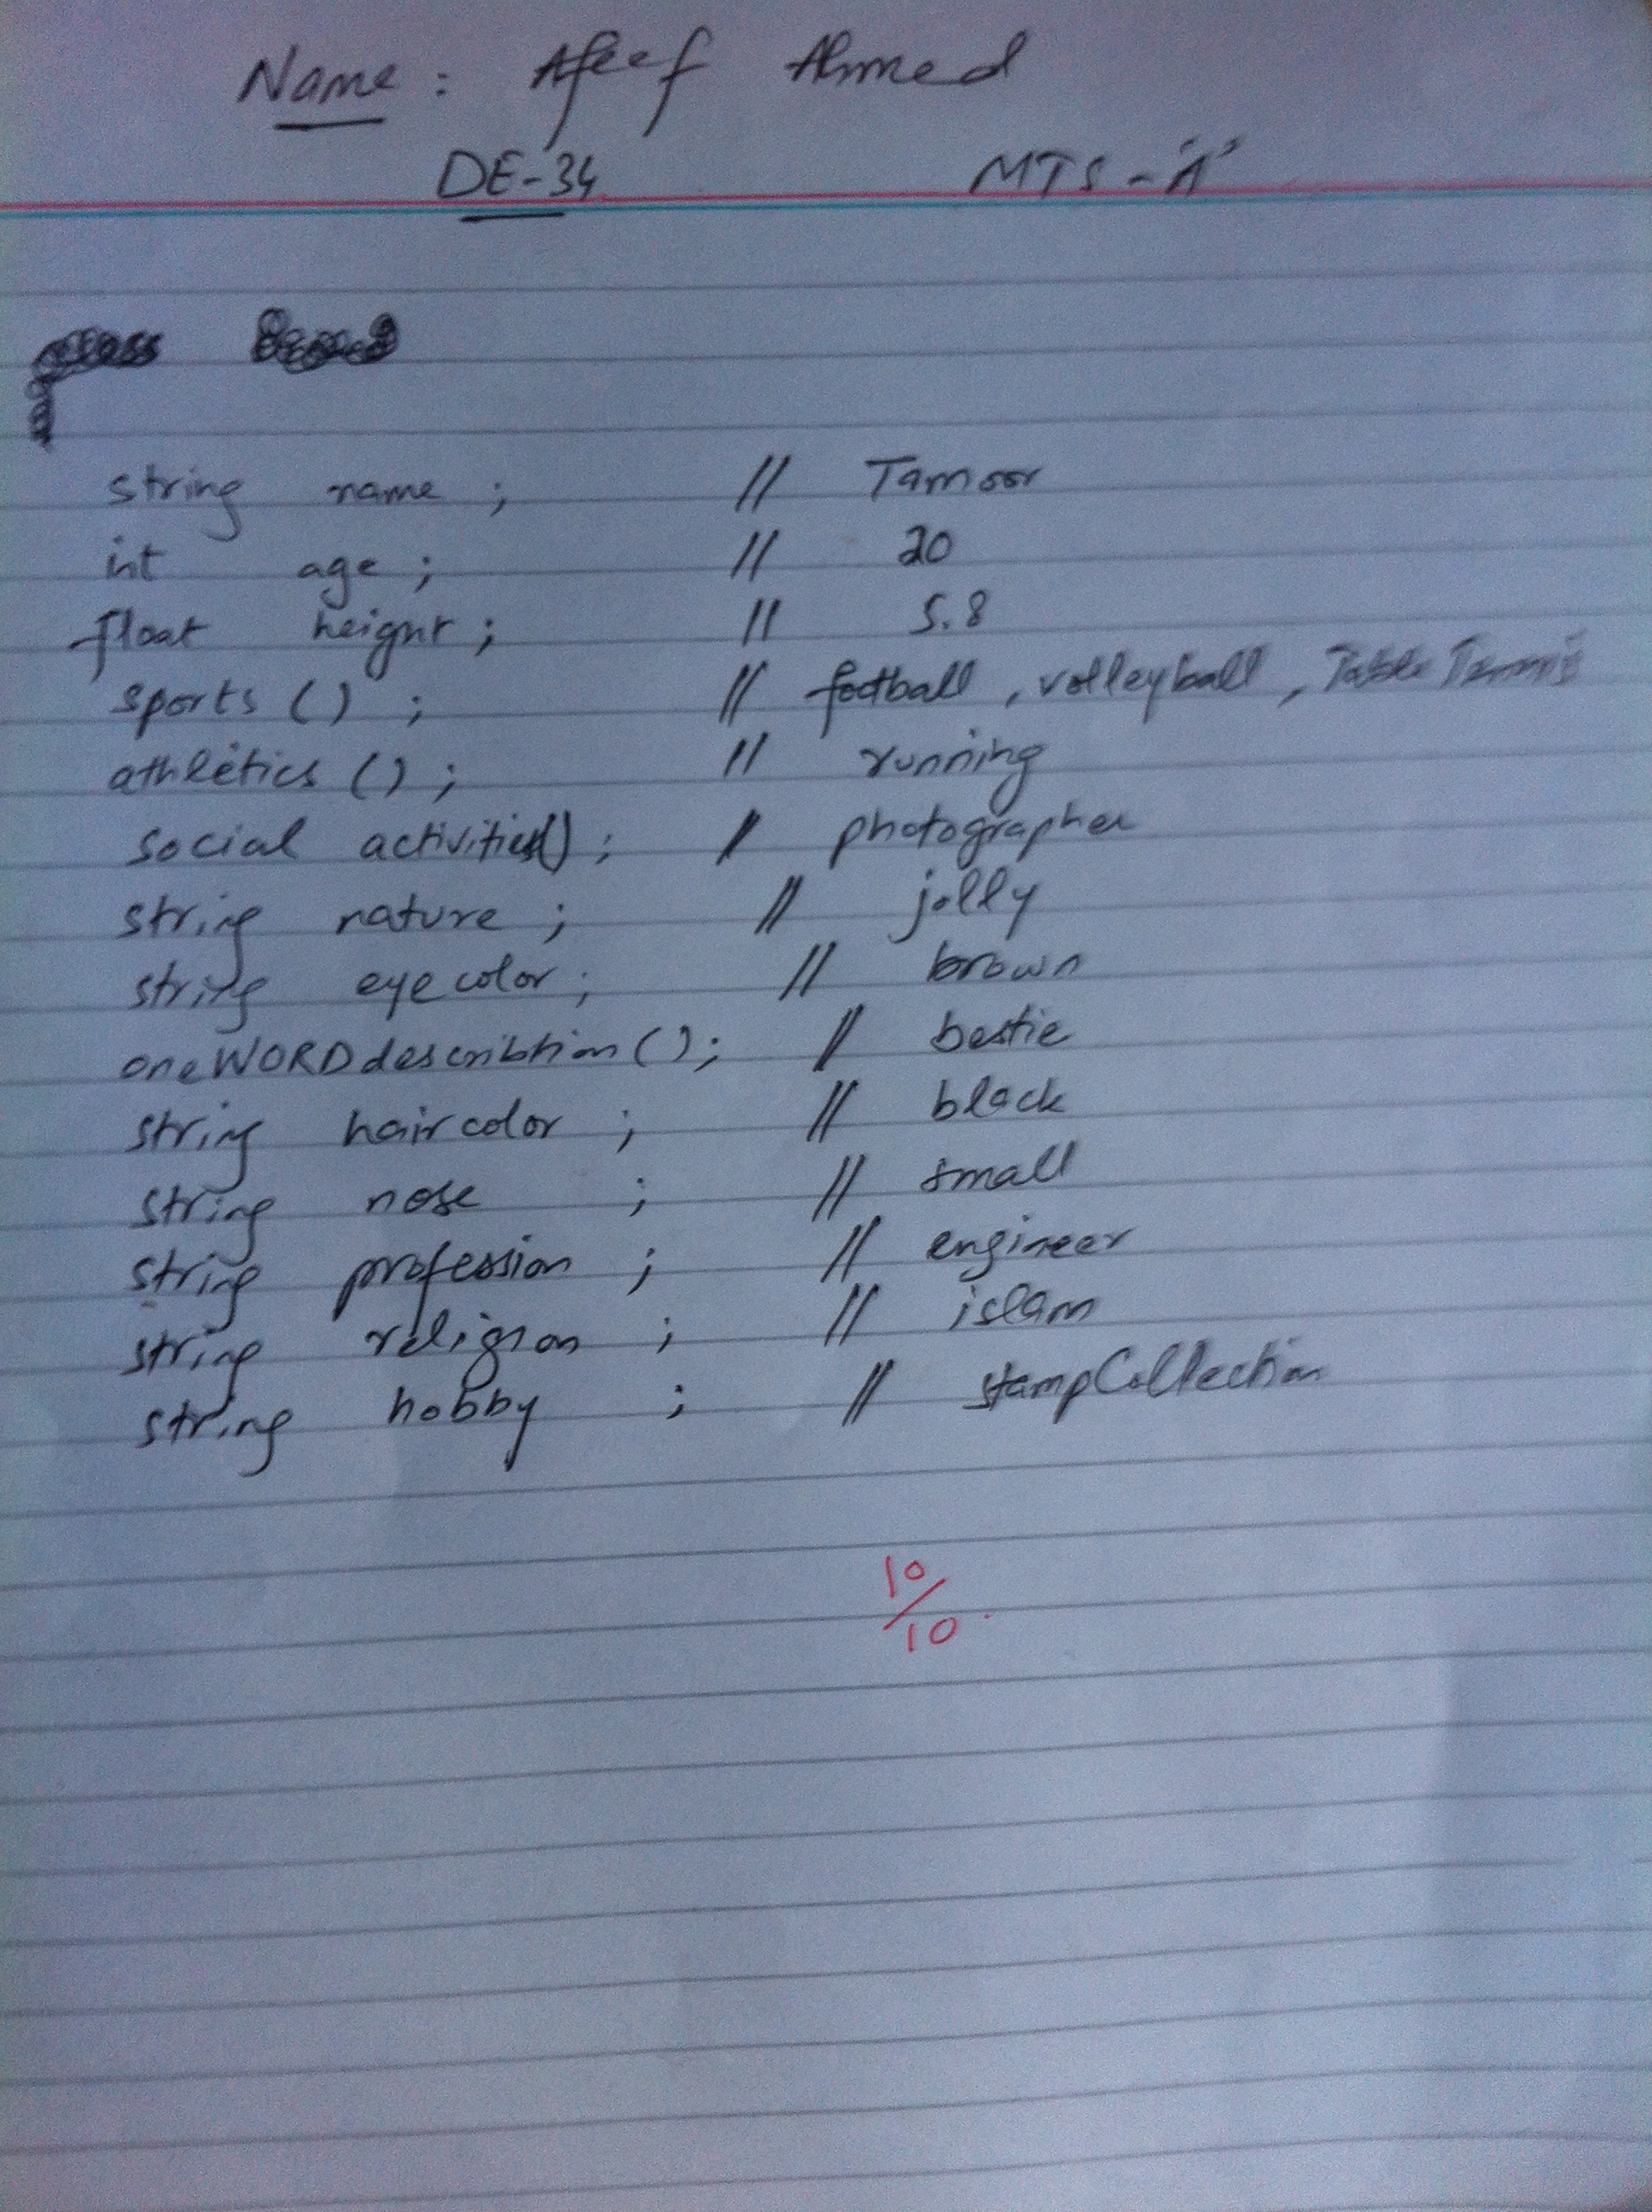
\includegraphics[width=0.4\columnwidth]{afeef}    
\caption{Afeef Ahmed}
  \end{figure}

}

\section{Operator Overloading}
\frame{\frametitle{Operator Overloading}
  \begin{itemize}
  \item<1-> Using Operators to perform different functions
  \item<2-> Built-in operators can be used with classes to perform Class specific tasks
  \item<3-> Similar concept to function overloading
   \end{itemize}
}

\begin{frame}[fragile]
\frametitle{Why Operator Overloading?}
\textbf{Synaptic Sugar: } Designed to make things easier to express and understand.
%\begin{small}
\begin{lstlisting}
Complex a(1.2,1.3);   
//this class is used to represent complex numbers  
Complex b(2.1,3);       
Complex c = a+b;        
//for this to work the addition operator must
// be overloaded
\end{lstlisting}
\end{frame}

\begin{frame}[fragile]
\frametitle{Operator Overloading Basic Example}
\Fontvi
\begin{lstlisting}
// vectors: overloading operators example
#include <iostream>
using namespace std;

class CVector {
  public:
    int x,y;
    CVector () {};
    CVector (int,int);
    CVector operator + (CVector);
};

CVector::CVector (int a, int b) {
  x = a;
  y = b;
}

CVector CVector::operator+ (CVector param) {
  CVector temp;
  temp.x = x + param.x;
  temp.y = y + param.y;
  return (temp);
}

int main () {
  CVector a (3,1);
  CVector b (1,2);
  CVector c;
  c = a + b;
  cout << c.x << "," << c.y;
  return 0;
}
\end{lstlisting}
\end{frame}
\begin{frame}[fragile]
\frametitle{Operator Overloading Basic Example}
Calling the overloaded operator.
\begin{lstlisting}
c = a + b;  //Implicit Calling
c = a.operator+ (b); //Explicit Calling
\end{lstlisting}
\end{frame}

\section{This Pointer}
\frame{\frametitle{This Pointer}
  \begin{itemize}
  \item ‘this’ pointer is passed as a hidden argument to all nonstatic member function calls
  \item Every object has access to its own address through this pointer.
  \item this$->$ member-identifier
  \end{itemize}
}
\begin{frame}[fragile]
\frametitle{This Pointer Example 1}
\begin{lstlisting}
class Something
{
private:
    int nData;
 
public:
    Something(int nData)
    {
        this->nData = nData;
    }
};
\end{lstlisting}
\end{frame}
\begin{frame}[fragile]
\frametitle{This Pointer Example 2}
\Fontvi
\begin{lstlisting}
#include <iostream>
using namespace std;
class Box
{
   public:
      Box(double l, double b, double h)
      {
         cout <<"Constructor called." << endl;
         length = l;
         breadth = b;
         height = h;
      }
      double Volume()
      {
         return length * breadth * height;
      }
      int compare(Box box)
      {
         return (this->Volume() < box.Volume());
      }
   private:
      double length;     // Length of a box
      double breadth;    // Breadth of a box
      double height;     // Height of a box
};

int main(void)
{
   Box Box1(3.3, 1.2, 1.5);    // Declare box1
   Box Box2(8.5, 6.0, 2.0);    // Declare box2
big = Box1.compare(Box2);
   return 0;
}
\end{lstlisting}
\end{frame}

\end{document}